\documentclass{article}
\usepackage{graphicx}                              %for PNG images (pdflatex)
\usepackage[linkbordercolor={1.0 1.0 0.0}]{hyperref} %for \url tag
\usepackage{color}                                 %for defining custom colors
\usepackage{framed}                                %for shaded and framed paragraphs
\usepackage{textcomp}                              %for various symbols, e.g. Registered Mark
\usepackage{geometry}                              %for defining page size
\usepackage{longtable}                             %for breaking tables
\usepackage{caption}
%
\geometry{verbose,a4paper,tmargin=2.5cm,bmargin=2.5cm,lmargin=2.5cm,rmargin=2cm}
\hypersetup{
  pdfauthor = {Ivan Marton, Peter Stefan},
  pdftitle = {The ARC gLite Gateway},
  pdfsubject = {ARC gLite gateway manual},
  pdfkeywords = {cream2, ARC1, Advanced Resource Connector, manual, users's manual, developers guide, gateway, gLite},
  pdfcreator = {PDFLaTeX with hyperref package},
  pdfproducer = {PDFLaTeX}
}
\bibliographystyle{IEEEtran}                       %a nice bibliography style
\def\efill{\hfill\nopagebreak}
\hyphenation{Nordu-Grid}
\setlength{\parindent}{0pt}
\setlength{\FrameRule}{1pt}
\setlength{\FrameSep}{8pt}
\addtolength{\parskip}{5pt}
%\renewcommand{\thefootnote}{\fnsymbol{footnote}}
\renewcommand{\arraystretch}{1.3}
\newcommand{\dothis}{\colorbox{shadecolor}}
\newcommand{\globus}{Globus Toolkit\textsuperscript{\textregistered}~2~}
\newcommand{\GT}{Globus Toolkit\textsuperscript{\textregistered}}
\newcommand{\ngdl}{\url{http://ftp.nordugrid.org/download}~}
\definecolor{shadecolor}{rgb}{1,1,0.6}
\definecolor{salmon}{rgb}{1,0.9,1}
\definecolor{bordeaux}{rgb}{0.75,0.,0.}
\definecolor{cyan}{rgb}{0,1,1}

\def\documenttitle{The glite gateway plugins of ARCLIB and related command line tools}
\captionsetup{margin=20pt,font={footnotesize, it},labelfont=bf}
\begin{document}
\def\today{\number\day/\number\month/\number\year}
\begin{titlepage}

\begin{tabular}{rl}
\resizebox*{3cm}{!}{
\includegraphics{logo-knowarc.png}}
\end{tabular}

\hrulefill

%-------- Change this to Knowarc_D<w>.<d>-<n>_<yy>

{\raggedleft DRAFT\_NORDUGRID-TECH-22\par}

{\raggedleft \today\par}

\vspace*{2cm}

%%%%---- The title ----
{\centering \textsc{\Large \documenttitle}\Large \par}
%\vspace*{0.5cm}
%%%%---- A subtitle, if necessary ----
{\centering \textit{\large Technical description and user manual}\large \par}
\vspace*{1.5cm}
%%%%---- A list of authors ----
{\centering \large Mattias Ellert\footnote{mattias.ellert@fysast.uu.se} \large \par}
{\centering \large Ivan Marton\footnote{martoni@niif.hu} \large \par}
{\centering \large Peter Stefan\footnote{stefan@niif.hu} \large \par}
%%%%---- An abstract - if style is article ----
%\begin{abstract}
%The abstract
%\end{abstract}
\end{titlepage}
\tableofcontents
\newpage
\section{Introduction}
\label{Introduction}
The purpose of this document is to describe this gLite\cite{glite} specific plugins of the ARCLIB (...Hivatkozni: jövőbeli Deliverable) to present the related command line utilities built on top of these libraries. The gateway library together with the tools enables seemless interoparability with gLite computing elements. It is possible, that relevant sections of this document will be moved into ARC1 userguide and into ARCLIB technical documentation. Interoperability with gLite storage element is provided by an other set of ARC library. This data library provides native interfaces to GridFTP\cite{gridftp} SRM which is the main bulding blocks of a gLite storage element. A storage interopability is out of scope of this library.
\section{Overview}
\label{Overview}
Interoperability has been one of the most important disciplines in recent grid middleware development. This term is often used in the sense of accessing resources operated by one kind of grid middleware (e.g. gLite) from a user interface operated by another kind (e.g. ARC1). There are two main possibilities to achieve this result:
\begin{itemize}
\item either to use a special infrastructure element, the gateway, which performs a full data structure and protocol translation between the two inter-operating grid middleware solutions,
\item or to explicitly implement the interface of the other side in the client.
\end{itemize}
The latter solution was preferred by ARC1 developers, the gLite gateway library module has been implemented in the ARCLIB and the gateway functionality will be transparently offered via the usual NorduGrid command line tools.\par
An overview of the preferred soulution is presented in figure \ref{fig:Chart 1}. The user will be able to express his requirements in the job description document using any of the xRSL\cite{xrsl}, JDL or JSDL\cite{jsdl} languages. The ARC client library will perform an automatic transformation. The gLite gateway functionality integrated into the ARCLIB, thus into the ARC client enables the user to transparently access gLite computing resources via the usual ARC command line tools. The gLite modules perform authentication, credential delagation and job submission to the CREAM2 CE. The CREAM2 CE may perform the necessary input file download from the different storage element. The library module gets job information through CREAM2 and sends management commands, like kill a job or undelegate credentials. Note, that not all the functionality described on the overview figure is implemented yet, for the current limitations see section \ref{Current limitations}!\par
\begin{figure}[ht]
\centering{\resizebox{\textwidth}{!}{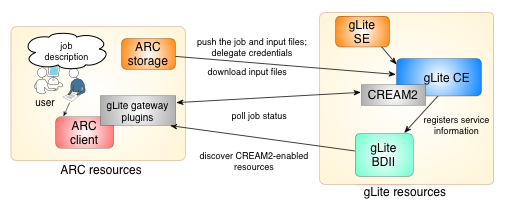
\includegraphics{D3-2-1-figure.png}}
\caption{\label{fig:Chart 1}This chart illustrates how the ARC1$\rightarrow$gLite gateway library module based approach works.}}
\end{figure}
\subsection{The supported gLite CE interface: CREAM2}
The gLite computing element (CE) offers several interfaces. Some of them are only suitabe for the WMS (glite resource broker) and was not meant to be used by 3rd party clients. Fortunately gLite comes with a webservice based computing element interface, known as the CREAM CE. The CREAM has undergone several major revisions. We can only hope that some stability will soon arise. The current CREAM version has entered the EGEE certification process newertheless it is a full scale deplomeyment on the EGEE worldwide grid has not taken place yet. CREAM2 is available on several preproduction and testing grid sites.\par
Nevertheless the KnowARC project chose the CREAM version 2\cite{cream} as the gLite computing element interface.\par
In particular, the gateway library was developed against version glite-ce-cream\_R\_1\_8\_3\_0\footnote{\url{http://grid.pd.infn.it/cream/field.php?n=Main.ReleaseNotes}}.\par
CREAM2 was chosen for the following reasons:
\begin{itemize}
\item CREAM2 has a web service interface that fits the web service based ARC1.
\item CREAM2 enables direct access to the gLite computing element without the need of going through the WMS.
\item CREAM2 contains numerous improvements compared to the earlier CREAM versions.
\item Unlike the other gLite CE interfaces it supports direct job status queries 
\item It is an official interface to gLite computing elements and as EGEE evolves it is expected that more and more computing elements will be deployed with CREAM2 interface.
\item CREAM2 offers a convenient way of handling input and output files through accessing the input and output sandbox via GridFTP.
\end{itemize}
In the near future CREAM will offer yet another interface which will be based on the BES/JSDL/GLUE OGF standards. This CREAM BES interface will coexists with the CREAM2 too.\par
\section{External dependencies and installation instruction}
\label{External dependencies and installation instruction}
The ARCLIB gLite plugins have only one dependency. GridFTP components of the Globus Toolkit\cite{globus} are needed to enable data staging functionality to those CREAM2 computing elements which offer input and output sandbox over a GridFTP enabled storage. Unfortunately the gateway library only works together with a strongly patched Globus verion. The NorduGrid patched Globus can be dowloaded from the NorduGrid download area\footnote{\url{http://download.nordugrid.org/software/globus/}}. Further information about the NorduGrid Globus patches can be read on the NorduGrid page\footnote{\url{http://wiki.nordugrid.org/index.php/Globus\_Libraries}}. It is worth to mention that the user will need a VOMS\cite{voms} proxy certificate in order to use the command line tools against a CREAM2 service. This VOMS proxy can be generated by using the VOMS client tools. It is only the VOMS enabled proxy certificate that is needed here, appart from this no VOMS component needed.\par
The ARC gLite gateway plugins library and the temporary command line utilities are incorporated into ARC1 releases. The source code is available from the ARC1 SVN repository\footnote{\url{http://svn.nordugrid.org/repos/nordugrid/arc1/}} and binary packages are provided at the NorduGrid download area. The build and installation instructions are given in the README file distributed together with the software. A step-by-step guide for Debian binary installation can be found in the appendix \ref{Debian install} \textit{Installation from Debian binary packages}.
\section{ARCLIB gLite gateway plugins}
\label{ARCLIB gLite gateway plugins}
The ARCLIB gLite gateway plugins constist of the wrapper classes, the job description handling facility and the gLite specific CREAMClient base class. The wrapper classes coveys the function provided by the CREAMClient to ARCLIB. The job description handling framework makes a general job request representation available for the other classes. CREAMClient base class implements the interface towards CREAM2 computing elements.
This client object has an easy-to-use and intuitive interface. It uses the VOMS proxy certificate to build the secure channel to the server and to sign that of the server's.
The different functions throw \textit{CREAMClientError} exceptions that should be caught in the application.\par
The following sections present the set of functions provided by the library.\par
\subsection{Wrapper classes}
... mik ezek a wrapper osztályok ... milyen base class, mit csinál, mi a funckiójuk ... viszonylag részletesen ...
\subsection{Job description translators}
... Bárhol meghívható ... objektumot példányosítani ... milyen transzformációk állank rendelkezésre ...
\subsection{CREAMClient base class}
\label{CREAMClient}
The client object uses the VOMS proxy certificate to build the secure channel to the server and to sign that of the server's.\par
... 1 bekezdés arról, hogy SOAP a hed(Hivatkozni!!!) SOAP framework-jét használja 'fully integrated'... az előző deliverable-ben a kommunikáció gSOAP-ot használt, ez az egyik nagy előrelépés, hogy ezt lecseréltük...\cite{gsoap}... 
\subsubsection*{CREAMClient(Arc::URL, Arc::MCCConfig)}
The constructor of the class performs the necessary initialization work. It receives two arguments: the service URL and the ARC message chain component configuration file to establish the communication channel to the server. These pieces of information are indispensable to create your client and to communicate with the remote site.
\subsubsection*{setDelegationId(std::string)}
Besides the constructor this is the other generic-purpose function that can be used in CREAM2 client applications. This function sets the previously registered and referred delegation ID on the client. The function is very simple: just set a private variable and returns with no value.
\subsubsection*{createDelegation(std::string)}
The \textbf{createDelegation} function is about to perform the whole delegation registration process. It sends a \textit{getProxyReq} message having the requested delegation ID, signs the received certificate and sends it back in a \textit{putProxy} SOAP message to the server. These three steps constitute the delegation registration process.
As almost every funtion, this one has no return value either. If there are any problems during the communication, either locally in the channel or at the remote site, the function throws \textit{CREAMClientError} described previously. If there are no exceptions thrown, then the command is considered to have successfully completed.
\subsubsection*{destroyDelegation(std::string)}
This method has the reverse functionality of the \textbf{createDelegation} function. It sends the \textit{destroy} message of CREAM2 to the remote server.
\subsubsection*{submit(std::string)}
The \textbf{submit} function is the most complex part of the class. It translates the job description received as the argument, registers the job with a \textit{JobRegisterRequest} message, uploads the locally stored files, if necessary, then enables the job execution on the server by sending a \textit{JobStartRequest} message. Finally it returns with a \textbf{creamJobInfo} object that contains a \textit{jobId} (job indetifier), a \textit{creamURL} (as the service URL), an \textit{ISB} (reference to the Input Sandbox) and an \textit{OSB} (Output Sandbox) member to describe the registered job. In the \textbf{glitesub} command (See Section \ref{glitesub} for details) these pieces of information are stored in the information file.
\subsubsection*{stat(std::string)}
This method queries the job status from the gLite CREAM2 server. The return value is the job status translated to the ARC terminology. The possible values are presented in the section of the \textbf{glitestat} command line tool. (See Section \ref{glitestat}!)
\subsubsection*{cancel(std::string)}
The \textbf{cancel} function sends a \textit{JobCancelRequest} SOAP message to the server and handles the emerging exceptions. It can be used for canceling a remotely registered and possibly running job.
\subsubsection*{purge(std::string)}
The \textbf{purge} function sends a \textit{JobPurgeRequest} message to server and throws an exception in case of any emerging problems.
\section{ARC command line tools for gLite CREAM2 CE}
\label{Users guide}
The well known ARC commands (ngsub, ngget, See: The NorduGrid/ARC User Guide\cite{userguide}!) will provide seemless access and integration with gLite computing elements. Full transparency will be achieved through the gLite gateway ARCLIB plugins. An ordinary user will use the same set of commands regardless of what type of CE to access. The user will be able to specify grid jobs described both in the gLite (JDL) and the NorduGrid (JSDL, xRSL) job description languages. The client will perform automatic conversion between the different job description languages.\par
Unfortunately the interoperability features offered by the gLite gateway library are not yet integrated into the NorduGrid commands. Also the current version of ARCLIB does not offer the full spectrum of language transformations.
However only a set of temporary command line tools exposing the available features of library are provided. These temporary commands make the already existing interoparabilily features usable for ordinary users.
There are seven different command line tools for using the gLite gateway functions. In this section these tools will be presented in detail through examples. The job descriptions and services shown are just simple examples, they might be different in real-life usage.\par
Every tool has a short manual page being accessible by using the \textbf{man} on-line manual reader command or some more help can be achieved by using the $<$command$>$ -? command line option.\par
\subsection{glitedelegate}
\label{glitedelegate}
In order to use gLite resources user must have a VOMS proxy. This proxy can be generated by command \textit{voms-proxy-init}.\par
For example:
\begin{shaded}\verb#$ voms-proxy-init -voms knowarc.eu#\end{shaded}
Once a VOMS proxy has been generated everything is in place to submit a new job. If one wants submit a job to a gLite server, first has to own a valid delegation on the remote site. This can either be an old, but still valid delegation identifier, or can be a new one. There is a command line tool to register a delegation on the CE to be used.\par
The usage of command \textbf{glitedelegate} is straighforward. All needed is a working CREAM2 delegation service URL, and a locally unique arbitrary delegation ID. This delegation ID will be associated to the remote resource. If you are not sure wether your favourite delegation ID is occupied or not, then try to delete it before registering it again. (See Section \ref{gliteundelegate} for further details!) The delegation command has the following syntax:
\begin{shaded}\verb#$ glitedelegate <delegation ID> <delegation service URL>#\end{shaded}
For example:
\begin{shaded}\verb#$ glitedelegate test_delegation \#\\*
\verb#        https://cream.grid.upjs.sk:8443/ce-cream/services/gridsite-delegation#\end{shaded}
\subsection{glitesub}
\label{glitesub}
The current command only supports direct job submission that is the user must know service endpoints. These kind of endpoints usually stored in LDAP databases. Ordinary ldapsearch can be used to find such an endpoint. Below an example:\par
\begin{shaded}
\verb#$ ldapsearch -x -h lxbra2305.cern.ch -p 2170 -b mds-vo-name=local,o=grid \#\\*
\verb#        '(GlueCEUniqueID=*cream*)' | grep GlueCEInfoContactString | \#\\*
\verb#        awk '{print $2}' | sort | uniq#
\end{shaded}
The \textbf{glitesub} command implements the actual job submission in three phases: registration of a job, uploading the local files to the input sandbox URL received during the registration and starting the job.\par
The \textbf{glitesub} command requires a valid delegation. See Section \ref{glitedelegate} how to create one. By the way this is the only command which needs the delegation ID.\par The next step is to prepare the necessary input files and the job description!\par
The glitesub command syntax is the following (please note that the service URL, job description, info file are mandatory and can only be given in the specified order):
\begin{shaded}\verb#$ glitesub -D <delegation ID> <service URL> <job description> <info file>#\end{shaded}
Here the delegation ID is the identification registered previously. The service URL will be different than in the delegation example above, because this is not the URL of the delegation, but the execution service. The job description must be in JDL format like in the example below. The info file stores information about the job submitted. It should either be a non-existing file otherwise it is overwritten. This file contains the job ID, the input sandbox URL, the output sandbox URL and the service URL.\par
Below I present a JDL description example. Note that the \textit{VirtualOrganisation} and \textit{QueueName} attributes should be the same as your virtual organisation name and the corresponding queue name on the server side.\par

\begin{minipage}{\textwidth}
\begin{framed}
\verb#[#\\
\verb#Executable = "/bin/hostname";#\\
\verb#StdInput = "std.in";#\\
\verb#StdOutput = "std.out";#\\
\verb#StdError = "std.err";#\\
\verb#BatchSystem = "pbs";#\\
\verb#VirtualOrganisation = "knowarc.eu";#\\
\verb#InputSandbox = {"std.in"};#\\
\verb#OutputSandbox = {"std.out","std.err"};#\\
\verb#QueueName = "knowarc.eu";#\\
\verb#OutputSandboxDestURI = { "gsiftp://localhost/std.out", "gsiftp://localhost/std.err" };#\\
\verb#]#
\end{framed}
\end{minipage}

An example how to use this command:
\begin{shaded}\verb#$ glitesub -D test_delegation \#\\*
\verb#        https://cream.grid.upjs.sk:8443/ce-cream/services/CREAM2 description.jdl job.info#\end{shaded}
... mit csinál a parancs sikeres és sikertelen futás esetén... \par
\subsection{glitestat}
\label{glitestat}
The \textbf{glitestat} command contacts to the CREAM2 service on the service URL and queries job status of a job specified by the job ID given in the info file.\par
Usage:
\begin{shaded}\verb#glitestat <info file>#\end{shaded}
For example:
\begin{shaded}\verb#glitestat job.info#\end{shaded}
The glitesub command implements a job status mapping between gLite and ARC job status semantics. The possible responses and their meanings are the following:
\begin{itemize}
\item ACCEPTING - the job submission is completed but the job is not yet scheduled
\item SUBMITTING - scheduling in progress
\item INLRMS:Q - the job is already at the local resource manager system and it is queued
\item INLRMS:R - the job is waiting at the local resource manager system for running
\item INLRMS:S - the job is running
\item KILLED - the job was terminated
\item FINISHED - the job has finished
\item FAILED - the job had some failure
\item FAILES - the job had some failure at LRMS level
\item EXECUTED - the job has been finished and there is no state information available
\end{itemize}
\subsection{glitekill}
\label{glitekill}
The \textbf{glitekill} command can be used for killing a remote job running in the underlying batch system. The only necessary argument needed is the information file made by \textbf{glitesub}. (See Section \ref{glitesub} for further details!) This command initiates stopping the job in the batch system. You can check the effect by using \textbf{glitestat}. (See Section \ref{glitestat} for its usage!)\par
Usage:
\begin{shaded}\verb#glitekill <info file>#\end{shaded}
For example:
\begin{shaded}\verb#glitekill job.info#\end{shaded}
\subsection{gliteclean}
\label{gliteclean}
Either after killing a job or because of some remote error occurs garbage files may remain on the server. These files can be purged by using command \textbf{gliteclean}. If you intentionally kill a job on the computing node, the job related stuff might also remain as garbage in the remote queue. This command also removes the job from the underlying batch system on the gLite computing element. It is important to note that this command removes the local information file as well. It might be useful to run this command after killing a job. (See Section \ref{glitekill}!)\par
Usage:
\begin{shaded}\verb#gliteclean <info file>#\end{shaded}
For example:
\begin{shaded}\verb#gliteclean job.info#\end{shaded}
\subsection{gliteundelegate}
\label{gliteundelegate}
After the work is complete it is possible to unregister and delete the delegation entry from the remote site by using command \textbf{gliteundelegate}. It can also be used when one needs to register a delegation ID but are unsure whether it is already used or not. Put the delegation delegation service URL into the argument!\par
Usage:
\begin{shaded}\verb#$ gliteundelegate <delegation ID> <delegation service URL>#\end{shaded}
For example:
\begin{shaded}\verb#$ gliteundelegate test_delegation \#\\*
\verb#        https://cream.grid.upjs.sk:8443/ce-cream/services/gridsite-delegation#\end{shaded}
\subsection{Skeleton of a temporary example gLite client}
Finally, here is an example code to present how easy and simple it is to write a new client using the CREAMClient class (See section \ref{CREAMClient}!). This code sample requests the job status of a previously submitted remote job, and writes it to the standard output. The client is written in C++.
\begin{framed}
\verb?#include "CREAMClient.h"?\\*
\verb?#include <iostream>?\\*
\\*
\verb?int main(int argc, char* argv[]){?\\*
\verb?  Arc::URL url( SERVICE_URL );?\\*
\verb?  Arc::MCCConfig cfg;?\\*
\\*
\verb?    Arc::Cream::CREAMClient gLiteClient(url,cfg);?\\*
\verb?    try {?\\*
\verb?        std::cout << "Job status: " << gLiteClient.stat( JOBID ) << std::endl;?\\*
\verb?    } catch (CREAMClienException& cce) {?\\*
\verb?        std::cerr << "ERROR: " << cce.what() << std::endl;?\\*
\verb?        return 1;?\\*
\verb?    }?\\*
\verb?    return 0;?\\*
\verb?}?
\end{framed}
It is of course mandatory to define \textit{SERVICE\_URL} and \textit{JOBID} strings to their real values to reach the proper functionality.
\section{Open issues}
In order to achieve the full scale transparent interoperability width the gLite computing element transparently offered through the NorduGrid client a couple of issues still need to be resolved. Most of these are related to the incomplete integration of the glite gateway library into the ARCLIB framework, even though the gateway library code is ready for production use. There are also some conceptual chanlenges due to the incompatible nature of the two systems which require development of some workarounds.
\subsection{Current limitations}
\label{Current limitations}
Full ARC1 client integration would mean that the temporary commands developed on top of the CREAMClient\ref{CREAMClient} presented in the previous section will be obsoleted by the ordinary ARC commands built on top of the ARCLIB. To achieve this the Wrapper class integration of the gLite gateway plugins library should finalized and exposed to extended testing.\par
Some of the Wrapper class methods and data structures should be extracted from the information available in the CREAMClient class. In particular, the detailed job representation needed for job monitoring is an open area.\par
The CREAMClient class will be extended to support operations such as SUSPEND available both in the CREAM2 interface and the ARCLIB's jobcontrol component.\par
Due to the incomplete ARCLIB integration currently only direct job submission to a manually selected CE is possible. The ARCLIB integration will combine the existing resource discovery (REF ... a Wrapperre) and job submission functionality (REF ... a Wrapperre)  of the glite gateway plugins with the brokering module of ARCLIB, which is  currently under development. The combination of these ARCLIB modules will provide intelligent brokered job submission over glite and nordugrid computing element.\par
For a fully transparent integration the automatic translation among JSDL/XRSL and JDL should also be provided. A user should be able to specify his/her job request in any of these languages and the gateway do the necessary translations.  The current language translator module currently is not capable generating JDL output.  Therefore, the user still needs to use JDL if he/she wants to submit jobs to CREAM2.\par
Further investigation is needed how a CREAM2 service handles data staging and whether the data movement related ARC libraries can be used to manage data staging in the client side or development of special data staging wrapper scripts to be executed on the computing element are needed.
A set of temporary workaround command line clients had to be developed (the glite* commands [... REF]) due to a discovered OpenSSL version conflict. The conflict appeared when we tried to integrate the CREAMClient gateway library with the rest of the ARCLIB. A tedious and time consuming debugging process took place. The debugging revealed the following:  A VOMS proxy certificate delegation method was implemented in the CREAMClient gateway library. During this process it was needed to sign a certificate and the original OpenSSL was used for this purpose. In the used communication library taken from the ARC1 framework there is a built-in Message Chain Component (MCC) which already utilizes the Globus Toolkit OpenSSL functions to enable establishing secure communication. Linking the CREAMClient library directly against the standard OpenSSL libs caused congesting SSL functions.  In order to resolve the OpenSSL conflict and to make possible the complete ARCLIB integration  a globus patch has been being worked on. Once the OpenSSL conflict is resolved the ARCLIB integration will be completed this way obsoleting the glite* temporary commands.\par
\subsection{Conceptional problems}
During the development of the gateway library a few conceptual incompatibilities were found.  These are the typical cases when one of the middlewares offers richer capabilities not available in the other one. These conceptual gaps can only be bridged by developing customized case by case workarounds, nevertheless  the interoperation always would result in some information loss in these cases.\par
Below we collected the most important challenges for which we still have to find some solution:
\subsubsection*{Expressing file staging in job description}
XRSL  offers reacher capability to describe input and output date of a job than the JDL.  Specifically, in xRSL it is possible for input files downloaded from storage servers to have their names changed. This is not possible in JDL. So a user might in xRSL ask for this:
\begin{shaded}
\verb#(inputfiles=(gsiftp://interop.dcgc.dk/storage/datafile1.txtinput.txt))#
\end{shaded}
That is not possible to express in JDL. It only allows the file to be downloaded as datafile1.txt. This could be solved by a wrapper script that renames files according to the xRSL specification. This does not solve our problem completely however. For example if a user wants to concatenate the stdout from two jobs, he would write something like the following in xRSL:
\begin{shaded}
\verb#(inputfiles=(gsiftp://interop.dcgc.dk/storage/job1/output.txtinput1.txt)#\\*
\verb#            (gsiftp://interop.dcgc.dk/storage/job2/output.txtinput2.txt))#
\end{shaded}
This cannot be solved just using the renaming method, because both input files would be retrieved before renaming is done and they would therefore overwrite each other.\par
A possible  solution is to recognize jobs of this type and simply barring them from using gLite resources or to let such jobs fail with an error message explaining that the user has to express their job in a different way.
\subsubsection*{RunTime Environments related issues}
Many grid jobs rely on software being available at the execution location. The requirement as well as the initialization of such software is expressed through the use of Run-Time Environments (RTEs). While the library is capable of translating the RTE request itself it is not capable of translating the name of the RTE. No standardized cross Grid nomenclature has been adopted, nor are the authors aware of any such activity. A temporary solution would be to have a remotely accessible list of RTEs and their names in each job description language. This could then be used for translating jobs.
\appendix
\section{Installation from Debian binary packages}
\label{Debian install}
This section contains instructions how to install the gateway libraries and glite* command line tools on Debian Linux.
\begin{enumerate}
\item Put the Debian repository into the APT source files (/etc/apt/sources.list). This repository in Luebeck is maintained as long as the KnowARC procject continues.
\begin{shaded}\verb#$ echo "deb http://pc02.inb.uni-luebeck.de:8080/~moeller/debian/stable ./" \#\\*
\verb#        >> /etc/apt/sources.list #\end{shaded}
\item Update the package list and install the necessary dependencies:
\begin{shaded}\verb#$ aptitude update#\\*
\verb#$ aptitude install voms globus globus-dev globus-doc#\end{shaded}
\item Add the Globus libraries to the system path:
\begin{shaded}\verb#$ echo "/opt/globus/lib" > /etc/ld.so.conf.d/globus.conf#\\*
\verb#$ ldconfig#\end{shaded}
\item Install ARC1 client.
\begin{shaded}\verb#$ aptitude install nordugrid-arc1-client#\end{shaded}
\item Create the vomses file:
\begin{shaded}\verb#$ mkdir -p /opt/glite/etc/#\end{shaded}
and copy these lines into the vomses file located at /opt/glite/etc/vomses
\begin{footnotesize}
\begin{shaded}
\verb#"gin.ggf.org" "kuiken.nikhef.nl" "15050" "/O=dutchgrid/O=hosts/OU=nikhef.nl/CN=kuiken.nikhef.nl" "gin.ggf.org"#\\*
\verb#"knowarc.eu" "arthur.hep.lu.se" "15001" "/O=Grid/O=NorduGrid/CN=host/arthur.hep.lu.se" "knowarc.eu"#\\*
\verb#"atlas" "voms.cern.ch" "15001" "/DC=ch/DC=cern/OU=computers/CN=voms.cern.ch" "atlas"#\\*
\verb#"nordugrid.org" "voms.uninett.no" "15015" "/O=Grid/O=NorduGrid/CN=host/voms.ndgf.org" "nordugrid.org"#\\*
\end{shaded}
\end{footnotesize}
\item Create \$HOME/.globus directory and move the user certificate-key pair into there.
\end{enumerate}
\bibliography{grid}
\end{document}
